\documentclass{my_Presentation}

\title{Agiles Softwaremanagement}
\author{Koch, Merkl, Pfitzner}
\institute{Mobile Robotic Laboratory}
\date{\today}

\begin{document}
%##################################################
\frame{\titlepage \vspace{-0.5cm}
\begin{center}
	
\includegraphics[scale=0.5]{Ohm.pdf}\\
	Technische Hochschule N�rnberg
\end{center}
}
%%~~~~~~~~~~~~~~~~~~~~~~~~~~~~~~~~~~~~~~~~~~~~~~~~~~~
\frame{
	\frametitle{Content}
	\begin{minipage}[b]{0.47\linewidth}
		\tableofcontents[pausesection]
	\end{minipage}
		\begin{minipage}[b]{0.47\linewidth}
	\begin{figure}
		
\includegraphics[width=\textwidth]{auton.png}
	\end{figure}
%	\begin{figure}
%		\includegraphics[width=\textwidth]{vb_comic.png}
%	\end{figure}
	\end{minipage}
	
}

%%##################################################
\section{Organisation}
\frame{
\frametitle{Teilnehmer}
	\begin{itemize}
		\item \textbf{Stefan May:} Product Owner
		\item \textbf{Philipp Koch:} Scrum Master
		\item \textbf{Christian Merkl:} Teammitglied
		\item \textbf{Christian Pfitzner:} Teammitglied
	\end{itemize}		
	\vfill
	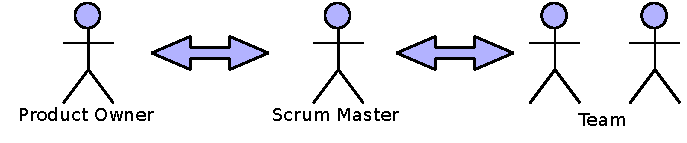
\includegraphics[width=0.9\textwidth]{../grafiken/Team.pdf}
 
}

%%##################################################
\frame{
\frametitle{Zeitplan}
	Gantt Diagramm
}

\section{Das Produkt}
\frame{
\frametitle{Das Produkt}
	\begin{block}{Eine grobe Idee}
		\begin{itemize}
			\item Handy-App
			\item Plattform f�r internationale Studenten
			\item Wichtige Informationen auf einen Blick
			\item Kommunikation untereinander
		\end{itemize}
	\end{block}
	\begin{flushright}
			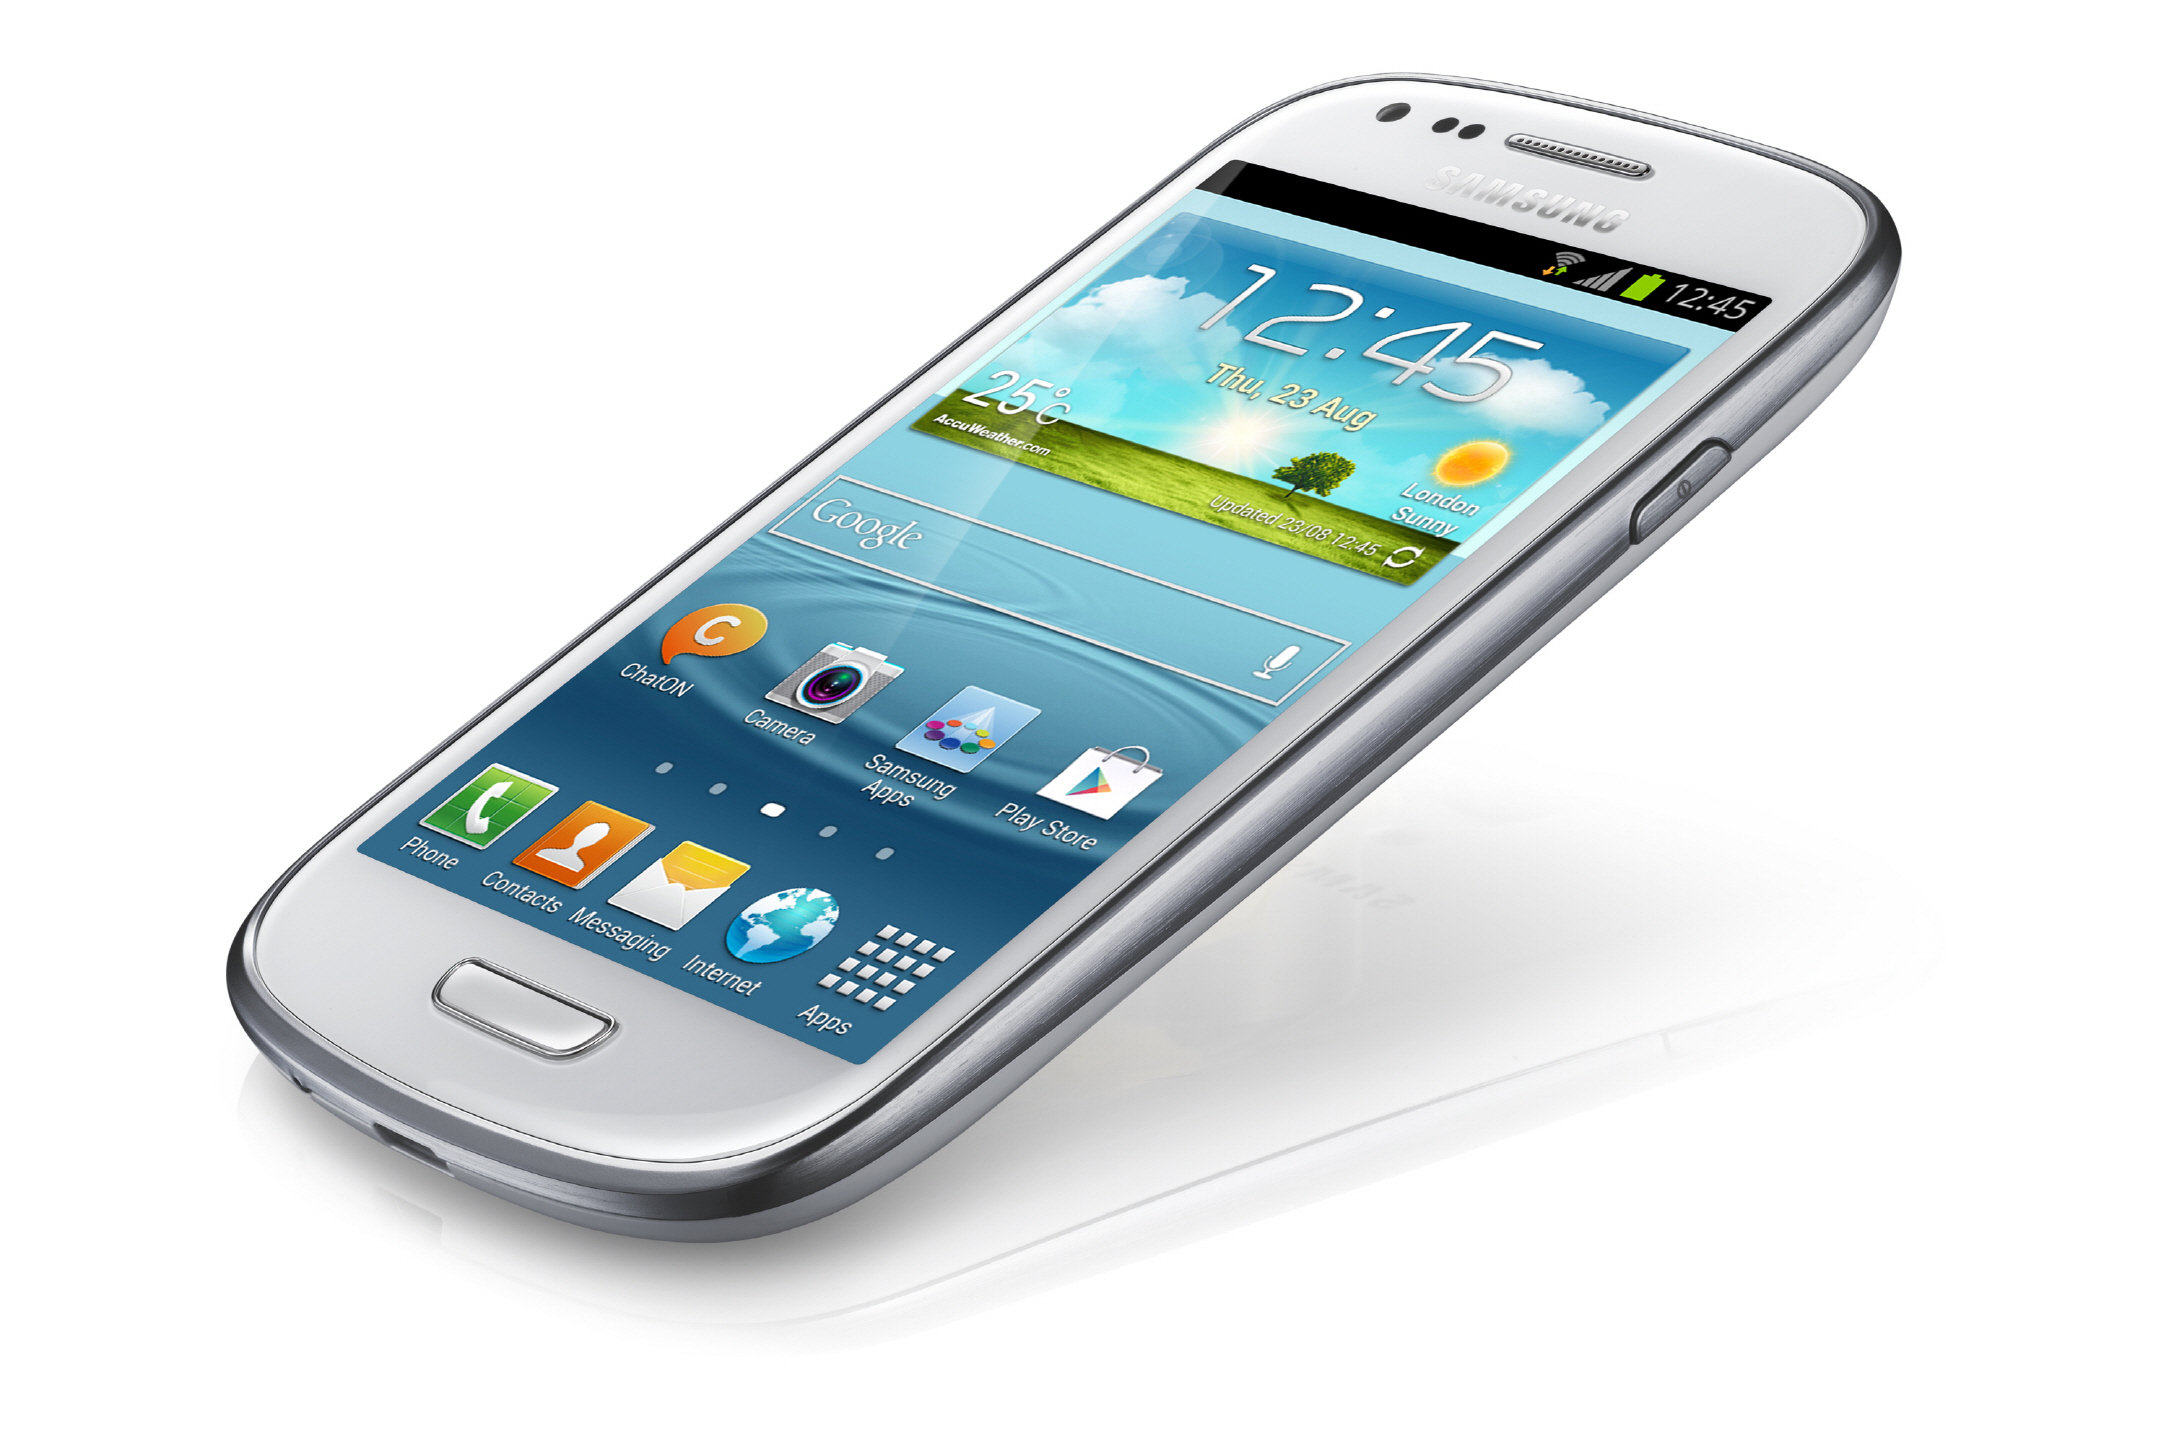
\includegraphics[width=0.5\textwidth]{../grafiken/s_handy.jpg}
	\end{flushright}
}

%%~~~~~~~~~~~~~~~~~~~~~~~~~~~~~~~~~~~~~~~~~~~~~~~~~~~
\section{Sprint 1}
\frame{
\frametitle{GUI: Programmaufbau}
	\begin{block}{Anforderungen}
		\begin{itemize}
			\item Basisklasse GUI enth�lt m�gliche Designelemente f�r einzelne Abschnitte der APP
			\item Seiten erben von Basisklasse und implementieren eigene Funktionalit�t
		\end{itemize}
	\end{block}
}

\frame{
\frametitle{Gui: Klassendiagramm}
	\begin{center}
			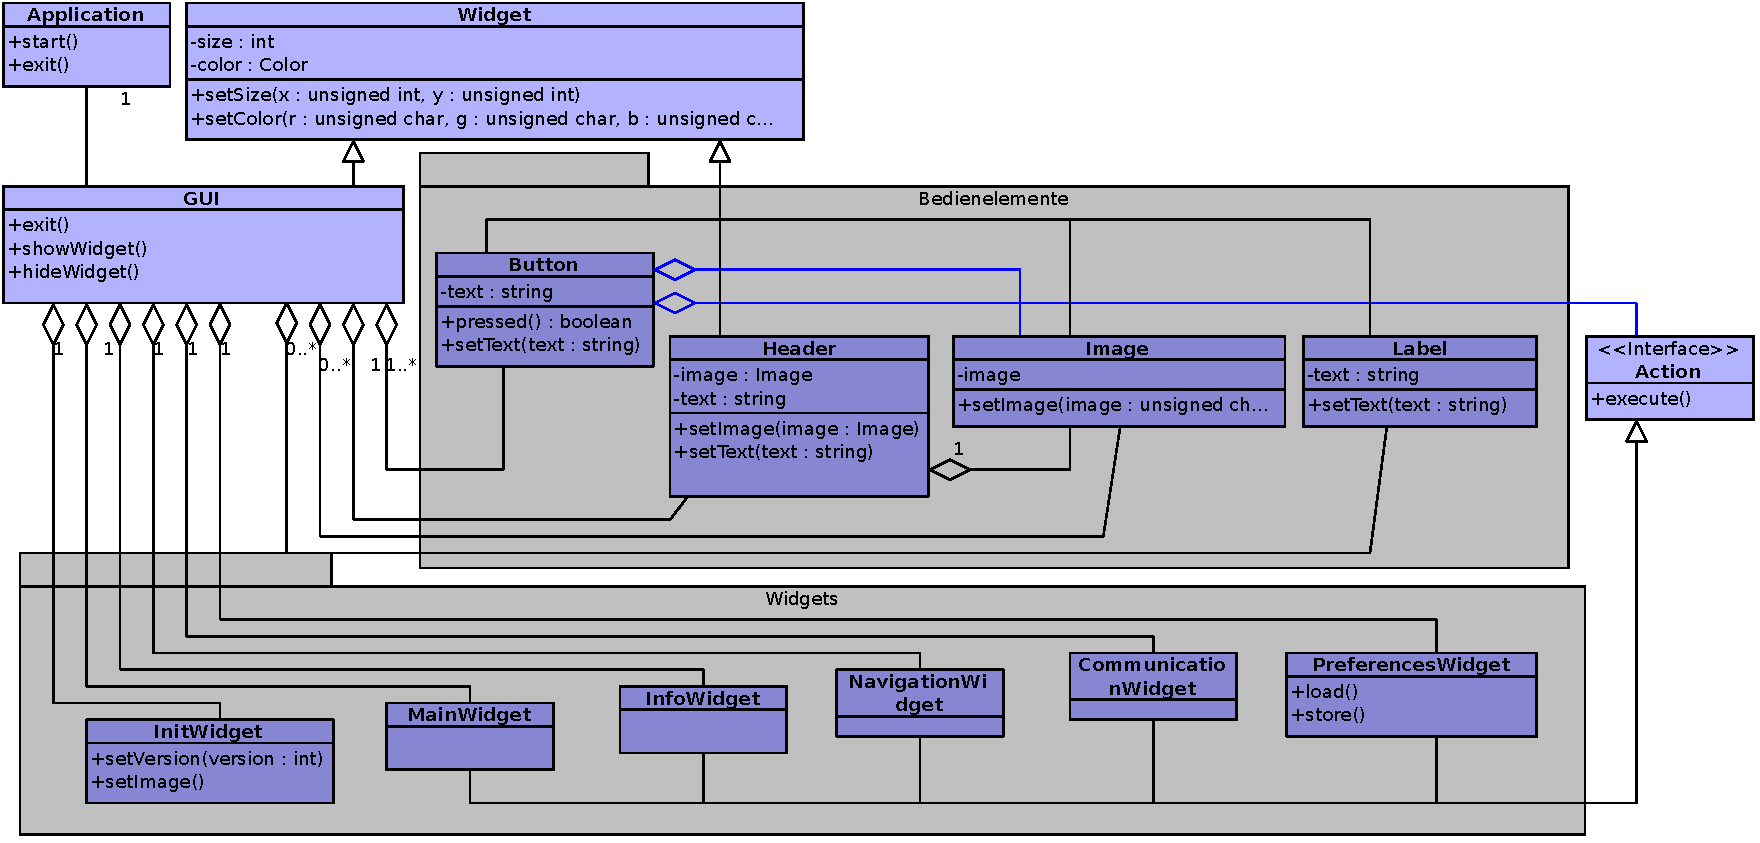
\includegraphics[width=0.9\textwidth]{../grafiken/GUI_Class.pdf}
	\end{center}
}


\frame{
\frametitle{Men�wechsel}
	\begin{block}{Zustandsmaschine}
		\begin{itemize}
			\item Men�punkte werden als Zustand gesehen
			\item zus�tzliche Zust�nde f�r Start und Beenden der Application
			\item Zust�nde k�nnen wiederum Unter-Zust�nde besitzen
		\end{itemize}
		\begin{center}
			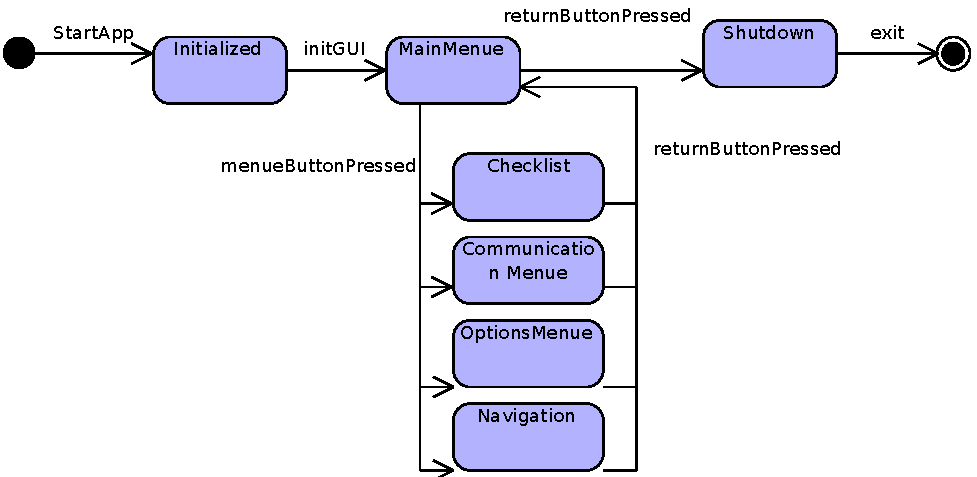
\includegraphics[width=0.8\textwidth]{../grafiken/MenueStates.pdf}
		\end{center}
	\end{block}
}




%%##################################################
\section{Sprint 2}
\subsection*{Datenhaltung: Backend}
\frame{
\frametitle{Hochschulkommunikation}
	\begin{block}{Kommunikation mit Hochschul-Content}
		\begin{itemize}
			\item Hochschule interne Daten �ber Content System
			\item Content-Zugriff bei Internetzugriff des Mobilfunktger�ts
		\end{itemize}
		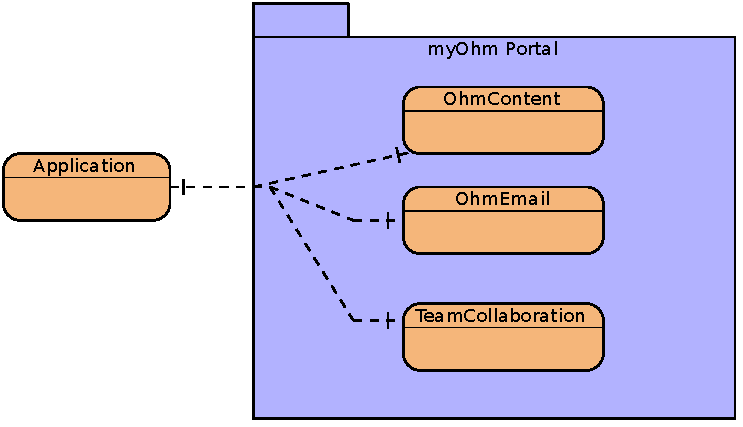
\includegraphics[width=0.9\textwidth]{../grafiken/OhmCollab.pdf}
	\end{block}
}

\frame{
\frametitle{Datenhaltung}
	\begin{block} {Content Management System (CMS)}
	\begin{itemize}
		\item CMS zum Verwalten von Inhalten
		\item Verschiedene Benutzerrollen:	
			\begin{itemize}
				\item Administrator: Bearbeitung von Design und Inhalt
				\item Redakteuer: Bearbeitung von Inhalt
			\end{itemize}
		\item $\rightarrow$ Hochschule benutzt bereits CMS Systeme f�r Inhalte der Webseite. \\\textbf{Vorteil: zus�tzliche Schulung nicht notwendig} 
	\end{itemize}
	\end{block}
	\begin{block} {Datenbank}
	\begin{itemize}
		\item mySQL-Datenbank	
		\item zyklisches Aktualisieren auf Endanwendung
	\end{itemize}
	\end{block}
}

\frame{
\frametitle{Zusammenspiel}
	\begin{block}{Diagramm}
		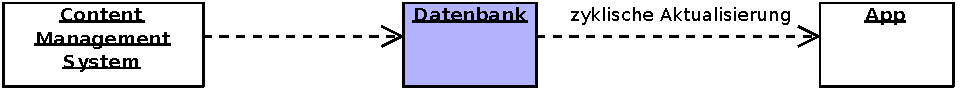
\includegraphics[width=1.0\textwidth]{../grafiken/DB.pdf}
	\end{block}
}

\subsection*{Navigation}
\frame{
\frametitle{Navigation: Struktur}
	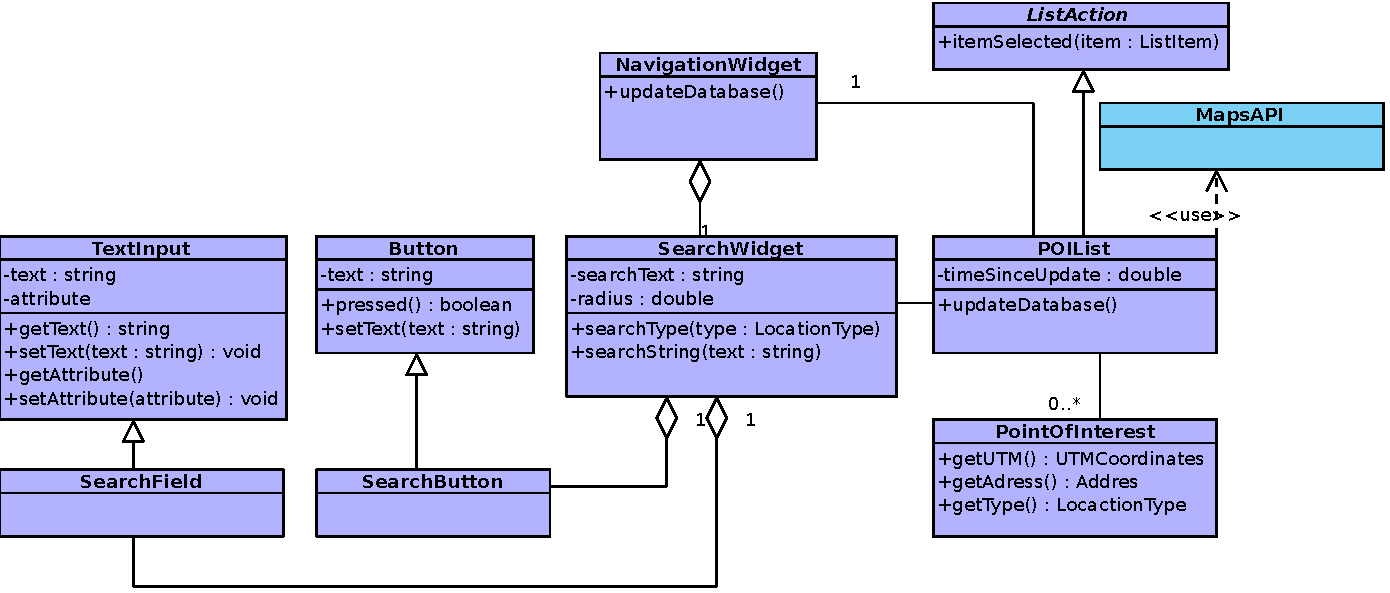
\includegraphics[width=0.9\textwidth]{../grafiken/NavigationW_Class.pdf}
}

\frame{
\frametitle{Interessantes}
	\begin{block}{Struktur}
	\begin{itemize}
		\item Basisklasse f�r interessante Objekte 
		\item Addressinformation f�r schnelles finden von Orten in der Umgebung
		\item UTM-Koordinaten zur �bergabe an Routenplanner
	\end{itemize}
	\begin{center}
		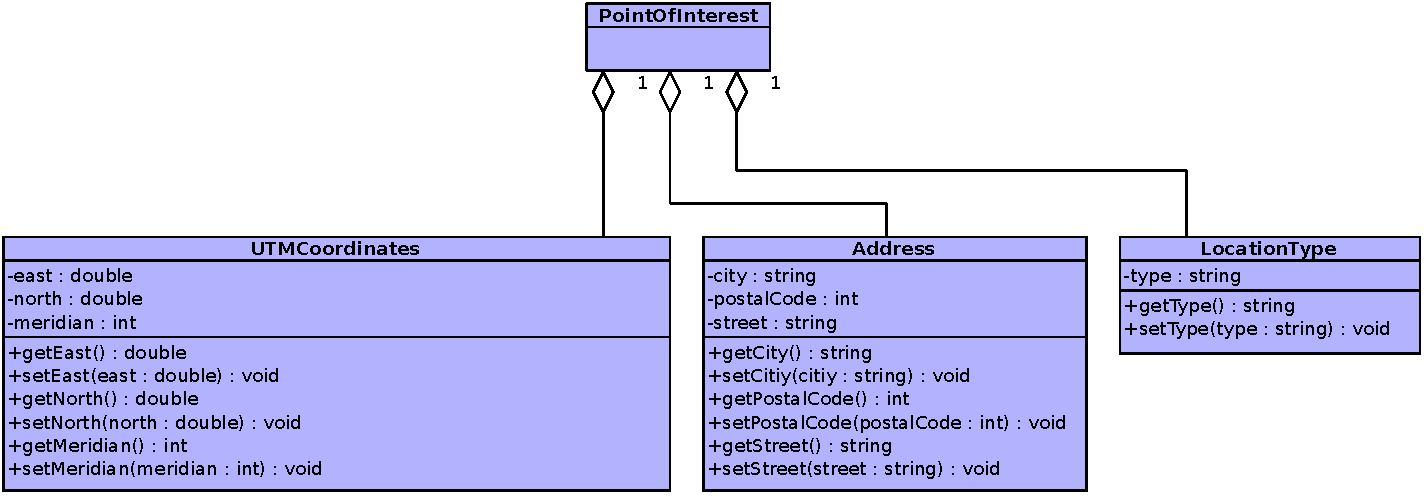
\includegraphics[width=0.8\textwidth]{../grafiken/PointOfInteresst.pdf}
	\end{center}
	\end{block}
}

%%##################################################


\section{Sprint3}

\section{Sprint4}

%%##################################################
\section{Ablauf}
\subsection*{Sprint 1}
%Sprint 1 user Story & Ablauf -> Phil
\frame{
\frametitle{Sprint 1 Hauptmenu - User Stories}
  \begin{block}{User Stories}
   \begin{itemize}
   \item Story 1 - Design
   
   Ich wuensche mir ein Menu, dass in Farbe und Form der Homepage meiner Hochschule aehnelt, dessen Bedienungsknoepfe links untereinander angebracht sind, welches eine Statusleiste mit den wichtigsten Informationen enthaelt und ein Foto des Nutzers zeigt.
   \item Story 2 - Funktionalitaet
   
   Ich moechte die Grundfunktionalitaet anhand von Dummyfunktionen sehen. 
   \end{itemize}
 \end{block}
}
\frame{
\frametitle{Sprint 1 Hauptmenu - Planung}
  \begin{block}{Extraktion aus Product Backlog}
   \begin{itemize}
   \item Design des Hauptmenu
    \item Design des Startbildes
    \item Implementierung der Grundfunktionalitaet (Dummy-Funktionen)
   \end{itemize}
  \end{block}  
}


%%##################################################

\subsection*{Sprint 2}
%Sprint 1 user Story & Ablauf -> Phil
\frame{
\frametitle{Sprint 2 Kartenwidget - User Stories}
  \begin{block}{User Stories}
   \begin{itemize}
   \item Story 1 - Lageplan TH
   
   Die App soll den Lageplan der Hochschule mit allen wichtigen Orten anzeigen.
   \item Story 2 - Google maps
   
   Die App soll eine Schnittstelle zu Google Maps enthalten.
   \item Story 3 - Interaktive Liste
   
   Der Nutzer soll Zugriff auf eine von ihm veraenderbare Liste mit fuer ihn interessanten Orten haben. 
   \item Story 4 - Darstellen von Orten aus der Liste
   
   In der Liste enthaltene Orte sollen in Google Maps dargestellt werden.
   \end{itemize}
 \end{block}
}

\frame{
\frametitle{Sprint 2 Kartenwidget - Planung}
  \begin{block}{Extraktion aus Product Backlog}
   \begin{itemize}
  	\item Lageplan der TH integrieren
    \item Interface zu Google-maps implementieren
    \item Implementierung interaktiver Liste fuer Kartenwidgets
    \item Uebergabe von Orten aus der Liste zu Google Maps
    \end{itemize}
  \end{block}
}


%%##################################################

\subsection*{Sprint 3}
%Sprint 3 user Story & Ablauf -> Phil
\frame{
\frametitle{Sprint 3 Kommunikation - User Stories}
  \begin{block}{User Stories}
   \begin{itemize}
   \item Story 1 - TH-Email / Kalender
   Die App soll eine Möglichkeit bieten, auf die Email- und Kalenderfunktionen der TH zuzugreifen.
   \item Story 2 - Reminder
   Die Statusleiste soll einen Reminder enthalten, welcher Termine anzeigt, die in einem im Optionsmenu einstellbaren Zeitfenster liegen.
   \item Story 3 - Popup
   Ein Popup soll Termine anzeigen, die in einem zweiten im Optionsmenu einstellbaren Zeitraum liegen. 
   \item Story 4 - Checklistenwidget
   Die App soll eine interaktive Checkliste enthalen, in die der Nutzer Aufgaben u. Ä. eintragen kann.
   \end{itemize}
 \end{block}
}

\frame{
\frametitle{Sprint 3 Kommunikation - Planung}
  \begin{block}{Extraktion aus Product Backlog}
    \begin{itemize}
    \item Schnittstelle zu TH-Email / Kalender implementieren
    \item Reminder in Statusleiste implementieren
    \item Popup fuer akute Termine implementieren 
    \item Implementierung des Checklistenwidgets
    \item Design des Reminders erstellen
    \item Design des Popups erstellen
    \item Design des Checklistenwidgets erstellen
    \end{itemize}
  \end{block}  

}

%%##################################################

\subsection*{Sprint 4}
%Sprint 4 user Story & Ablauf -> Phil
\frame{
\frametitle{Sprint 4 Redesign - User Stories}
  \begin{block}{Entscheidung des PO - Name der Hochschule wurde geändert}
  \end{block}
  \begin{block}{User Stories}
   \begin{itemize}
   \item Story 1 - Aenderung des Logos und der Schriftzüge
   
   Ich wünsche mir, dass die Logos und Schriftzüge in den Widgets an den neuen Namen der TH angepasst werden.
   
   \item Story 2 - Redesign des Startbildschirms
  
   Der Startbildschirm der App soll an den neuen Namen der TH angepasst werden.
   \end{itemize}
 \end{block}
}

\frame{
\frametitle{Sprint 4 Redesign - Planung}
  \begin{block}{Extraktion aus Product Backlog}
    \begin{itemize}
    \item Aenderung der Logos und der Schriftzüge in allen Widgets
    \item Redesign des Startbildschirms
    \end{itemize}
  \end{block}   
}

%%################################################## 

\subsection*{Sprint 5}
%Sprint 5 user Story & Ablauf -> Phil
\frame{
\frametitle{Optionsmenü - User Stories}
  \begin{block}{User Stories}
   \begin{itemize}
   \item \textbf{Funktionen des Optionsmenü: }\textit{Die App soll ein Optionsmenü enthalten, in dem sich alle für den Nutzer relevanten Einstellungen verändern lassen. }
   \item \textbf{Design des Menü-Widgets: } \textit{Das Menüwidget soll Buttons enthalten, die genauso aussehen, wie die im Hauptmenü. Die Buttons sollen gleichmäßig über den Bildschirm verteilt werden. }
   \end{itemize}
 \end{block}
}

\frame{
\frametitle{Optionsmenü}
  \begin{block}{Extraktion aus Product Backlog}
    \begin{itemize}
    \item Implementierung aller Funktionen des Optionsmenu
    \item Design des Menü-Widgets
    \end{itemize}
  \end{block}   
}

%%################################################## 

\subsection*{Sprint 6}
%Sprint 6 user Story & Ablauf -> Phil
\frame{
\frametitle{Sprint 6 Partnerhochschulen - User Stories}
  \begin{block}{Entscheidung des PO - Partnerhochschulen sollen App mitverwenden können}
  \end{block}
  \begin{block}{User Stories}
   \begin{itemize}
   \item Story 1 - Variables Widgetdesign
   \item Story 2 - Variable Datenbankanbindung
   \item Story 3 - Variable Datenbankanbindung
   \item Story 4 - Erweitertes Optionsmenu   
   \end{itemize}
 \end{block}
}

\frame{
\frametitle{Sprint 6 Partnerhochschulen - Planung}
  \begin{block}{Extraktion aus Product Backlog}
    \begin{itemize}
    \item Design aller Widgets variabel
    \item Datenbankanbindung variabel
    \item Hochschullageplan variabel
    \item Optionsmenu erweitern
    \end{itemize}
  \end{block}  
  
}


%\item Story 1 - Aenderung der Logos
%   
%   Ich wünsche mir, dass die Logos in den Widgets sich an die Logos unserer Partnerhochschulen anpassen lassen.
%   \item Story 2 - Aenderung der TH-Schriftzuege
%   
%   Die Schriftzüge in den Widgets sollen sich an den Namen der Partnerhochschulen anpassen lassen.
%   \item Story 3 - Redesign des Startbildschirms und aller Widgets
%   
%   Der Startbildschirm und alle Widgets der App sollen sich dem Design der Homepage der jeweiligen Partnerhochschule anpassen lassen.

%%################################################## 

\section{Fazit}
\frame{
\frametitle{Lessons Learned}
	\begin{block}{Was lief gut?}
		\begin{itemize}
			\item erster Punkt
		\end{itemize}
	\end{block}
	\begin{block}{Was lief schlecht?}
		\begin{itemize}
			\item erster Punkt
		\end{itemize}
	\end{block}
}

%%~~~~~~~~~~~~~~~~~~~~~~~~~~~~~~~~~~~~~~~~~~~~~~~~~~~
\frame{
\frametitle{Thank you for your attention}
	\begin{block}{Contact}
	\flushright{
	\tiny Title.\\ \normalsize
	\textbf{Name} \\
	Laboratory of mobile Robotics\\
	Kesslerplatz 12 -- KA 640\\
	90489 Nuremberg \\
	\url{Email40432@ohm-hochschule.de}
	}
	\end{block}	
	\begin{figure}
		
\includegraphics[width=0.5\textwidth]{auton.png}
	\end{figure}
}

%##################################################
\frame{%\section*{References}
\frametitle{References}
	\begin{block}{Verwendete Software}
			\begin{itemize}
				\item Eclipse Kepler 
				\item Visual Paradigm for UML Professional Edition
			\end{itemize}
	\end{block} 
		
	References

}
\end{document}
